\documentclass[12pt, a4paper]{article} 
 
\usepackage[utf8]{inputenc}
 
 
\usepackage{geometry} % to change the page dimensions
\geometry{a4paper} % or letterpaper (US) or a5paper or....
 
\usepackage{graphicx} % support the \includegraphics command and options
 
\usepackage{booktabs} % for much better looking tables
\usepackage{array} % for better arrays (eg matrices) in maths
\usepackage{paralist} % very flexible & customisable lists (eg. enumerate/itemize, etc.)
\usepackage{verbatim} % adds environment for commenting out blocks of text & for better verbatim
\usepackage{subfig} % make it possible to include more than one captioned figure/table in a single float
% These packages are all incorporated in the memoir class to one degree or another...
 \usepackage{import} % for importing other .tex files
 
 
\usepackage{amsmath, amssymb}% for mathematical symbols
\usepackage[colorlinks=true,linkcolor=black]{hyperref} % for hyperreferences with black color
\usepackage[T1]{fontenc} % Uncomment for norwegian document
%\usepackage[norsk]{babel} %
 
%%% HEADERS & FOOTERS
\usepackage{fancyhdr} % This should be set AFTER setting up the page geometry
\pagestyle{fancy} % options: empty , plain , fancy
\renewcommand{\headrulewidth}{0pt} % customise the layout...
\lhead{}\chead{}\rhead{}
\lfoot{}\cfoot{\thepage}\rfoot{}
 
%%% SECTION TITLE APPEARANCE
\usepackage{sectsty}
\allsectionsfont{\sffamily\mdseries\upshape} % (See the fntguide.pdf for font help)
% (This matches ConTeXt defaults)
 
%%% ToC (table of contents) APPEARANCE
\usepackage[nottoc,notlof,notlot]{tocbibind} % Put the bibliography in the ToC
\usepackage[titles,subfigure]{tocloft} % Alter the style of the Table of Contents
\renewcommand{\cftsecfont}{\rmfamily\mdseries\upshape}
\renewcommand{\cftsecpagefont}{\rmfamily\mdseries\upshape} % No bold!

%%%Code
\usepackage{color}
\definecolor{bluekeywords}{rgb}{0.13,0.13,1}
\definecolor{greencomments}{rgb}{0,0.5,0}
\definecolor{redstrings}{rgb}{0.9,0,0}

\usepackage{listings}
\lstset{language=[Sharp]C,
showspaces=false,
showtabs=false,
breaklines=true,
showstringspaces=false,
breakatwhitespace=true,
escapeinside={(*@}{@*)},
commentstyle=\color{greencomments},
keywordstyle=\color{bluekeywords}\bfseries,
stringstyle=\color{redstrings},
basicstyle=\ttfamily
}
 
 
 
%%% END Article customizations
 
%%% The "real" document content comes below...
 
\title{\normalsize Customer driven project, TDT4290 \\ \LARGE \textbf{Automatic Import of Completed Ads} \normalsize \\Adresseavisen AS}
\author{Audun Skjervold \\ Erlend Løkken Sigholt \\ Truls Hamborg \\ Hong-Dang Lam}
%\date{} % Activate to display a given date or no date (if empty),
         % otherwise the current date is printed 
 
\begin{document}
\maketitle 
\newpage
\tableofcontents
\newpage

\chapter*{Abstract}

This paper describes the process of developing a framework for Automatic Importing of Completed Ads, on request from Adresseavisen AS, which is a major regional newspaper. It will describe the project, from the preliminary study phase and project management/organization, to implementation and completion.

The goal is to create a framework which will facilitate automatic importing of completed real estate ads in the form of pdf-files and associated data, with the possibility to expand to other types of ads. The accompanying data will be placed into the internal database of Adresseavisen and their internal order system for ads, and the pdf is to be saved in their archives.

Adresseavisen, as a customer, is interested in the framework in itself, with accompanying developer documentation for possible further development. In addition to this, we will produce full documentation of the process as a deliverable in the course which this project is for.

\chapter*{Preface}
This document was written for the project-based course \em TDT4290 Customer Driven Project\em, at the \em Norwegian University of Technology and Science, NTNU\em \ during the fall semester of 2013.

The project team consisted of four students from \em Computer Science \em  at the \em Department of Computer and Information Science\em \ at \em NTNU\em. The project was \em Automated Import of Completed Ads\em, on behalf of \em Adresseavisen AS\em.

The team would like to thank customer representative Asle Dragsteen Liebech for great support and technological guidance, as well as our supervisor Zhu Meng for excellent supervising.
 
\section{Introduction}
\subsection{Project name - Automatic Import of Completed Ads}
\subsection{Customer - Adresseavisen AS}
\subsection{Project background}
\subsection{Problem Description}
\subsection{Stakeholders}
\subsection{Measure of Project Effects}
\subsection{Duration}

\subsection{Report outline}

\section{Project Management}
\subsection{Terms and Resources}
\subsection{Project Organization}
\subsection{Roles}
\documentclass[12pt, a4paper]{article} 
 
\usepackage[utf8]{inputenc}
 
 
\usepackage{geometry} % to change the page dimensions
\geometry{a4paper} % or letterpaper (US) or a5paper or....
 
\usepackage{graphicx} % support the \includegraphics command and options
 
\usepackage{booktabs} % for much better looking tables
\usepackage{array} % for better arrays (eg matrices) in maths
\usepackage{paralist} % very flexible & customisable lists (eg. enumerate/itemize, etc.)
\usepackage{verbatim} % adds environment for commenting out blocks of text & for better verbatim
\usepackage{subfig} % make it possible to include more than one captioned figure/table in a single float
% These packages are all incorporated in the memoir class to one degree or another...
 
 
 
\usepackage{amsmath, amssymb}% for mathematical symbols
\usepackage[colorlinks=true,linkcolor=black]{hyperref} % for hyperreferences with black color
%\usepackage[T1]{fontenc} % Uncomment for norwegian document
%\usepackage[norsk]{babel} %
 
%%% HEADERS & FOOTERS
\usepackage{fancyhdr} % This should be set AFTER setting up the page geometry
\pagestyle{fancy} % options: empty , plain , fancy
\renewcommand{\headrulewidth}{0pt} % customise the layout...
\lhead{}\chead{}\rhead{}
\lfoot{}\cfoot{\thepage}\rfoot{}
 
%%% SECTION TITLE APPEARANCE
\usepackage{sectsty}
\allsectionsfont{\sffamily\mdseries\upshape} % (See the fntguide.pdf for font help)
% (This matches ConTeXt defaults)
 
%%% ToC (table of contents) APPEARANCE
\usepackage[nottoc,notlof,notlot]{tocbibind} % Put the bibliography in the ToC
\usepackage[titles,subfigure]{tocloft} % Alter the style of the Table of Contents
\renewcommand{\cftsecfont}{\rmfamily\mdseries\upshape}
\renewcommand{\cftsecpagefont}{\rmfamily\mdseries\upshape} % No bold!

\begin{document}

\section{Roles}
\begin{itemize}
\item Scrum Master/Process responsible: Truls
\item Documentation Manager: Truls
\item Product Owner: Adresseavisen
\item Customer/Supervisor contact: HD
\item Administrator/Project Leader, System Architect: HD
\item Lead Coder, Project Lead: Erlend
\item Secretary: Erlend
\item Implementation manager: Audun
\end{itemize}


Test Manager: Everyone is responsible for testing their own code.


\end{document}
\subsection{Time schedule}
\subsection{Overall project plan}
\subsection{Risk Analysis}
\subsubsection{Internal Risks}
\subsubsection{External Risks}
\subsection{Procedures for Quality Assurance}

\section{Preliminary Studies}
\subsection{Development Methodology}
\subsubsection{Waterfall}
\subsubsection{Scrum}
\subsubsection{What we have chosen}
\subsection{Frameworks}
\subsubsection{Software Development Model}
\subsubsection{Programming languages, Communication Protocols and File Formats}
\subsubsection{Web Api}
\subsubsection{Server}
\subsubsection{Database}
\subsection{Extra Tools}
\subsection{Existing Technology}
\subsection{Standards}
\subsection{Summary}

\section{Requirements Specification}


%Architecture
\section{Architecture}
\label{Architecture}
\subsection{Stakeholders}

\subsubsection{Customer}
Our goal with this course was to create a product that not only works the way the customer intended, but does so with satisfactory performance. It also needed a clear, logical and functional architecture to make it easy to maintain. 
Our code needed to be written following the clean coding standard and make use of interfaces and general polymorphism, so that their developers could further develop this solution with ease.

\subsubsection{Implementers}
We wanted an architecture that would be easy to implement and would make sense to the coders of our own team as well as to those of the customer.

\subsubsection{Course Staff}
The course staff wants a clear and well-documented architecture that is easy to understand and evaluate.


\subsection{Quality Attributes}
The customer was very specific when it came to what they wanted. % Were they, though? Rewrite/elaborate

\subsubsection{Modifiability}
While we were the create the solution for real estate ads specifically, the solution will be used for other ads as well. Therefore we need to make it modifiable so that other developers later on can further develop using our solution as a base.

\subsubsection{Performance}
We wanted the system to function with a satisfactory performance, even though the customer did not set any specific requirements for performance. For this reason, we decided to merely strive to achieve this goal by writing as efficient code as we could manage, making necessary changes to keep performance at a reasonable level. %Is this too vague?

\subsubsection{Availability}
The system should be available for the users when they need it. Therefore we needed to minimize the possible points of failure and the probability of these failing. % Too vague?

\subsubsection{Interoperability}
Our solution was only a part of the larger Webassistenten solution, and needed to inter-operate with already-existing order system. To achieve this goal, we used the same technology as requested by the customer, including Web API, MSSQL and so on.

\subsubsection{Readability}
The customer wants us to write readable code. The customer wants us to write interfaces and using polymorphism so other developers can develop it further by developing plug-ins for the system. Readability is therefore important for easier further development of this system.
%Whoever wrote this should probably rewrite it.

\subsection{Views}


\subsubsection{Process view}
There is no need for us to supply a process view, because we do not have access to their server. We are only supposed to write the code for their system, without taking into account how the processes inter-operate.
\subsubsection{Logical view}
\begin{figure}[H]
\centering
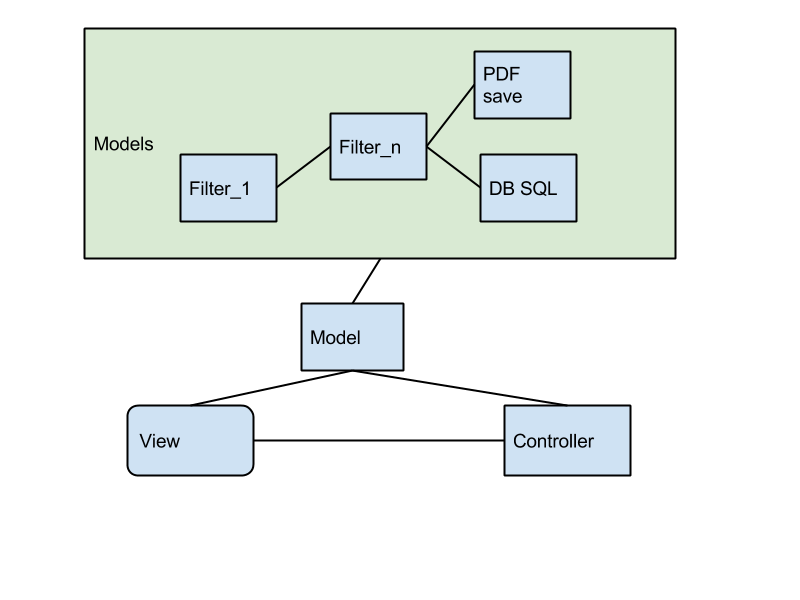
\includegraphics[width=0.8\textwidth]{images/architecture00.png}
\caption{Logical view}
\label{fig:logical_view}
\end{figure}
\newpage

\subsubsection{Scenario view}
\begin{figure}[H]
\centering
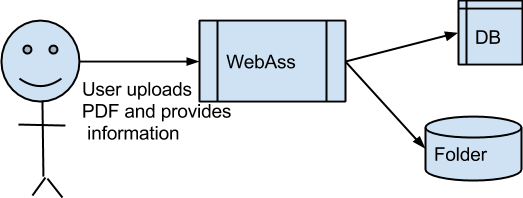
\includegraphics[width=0.8\textwidth]{images/architecture01.png}
\caption{Scenario view}
\label{fig:scenario_view}
\end{figure}




\subsubsection{Physical view}
\begin{figure}[H]
\centering
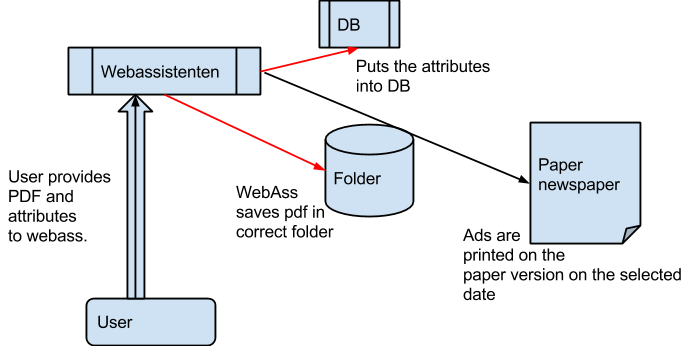
\includegraphics[width=0.8\textwidth]{images/architecture02.png}
\caption{Physical view, we implement the red arrows}
\label{fig:physical_view}
\end{figure}
\newpage
\subsection{Class diagram}
From these views, we made this class diagram.
\begin{figure}[H]
\centering
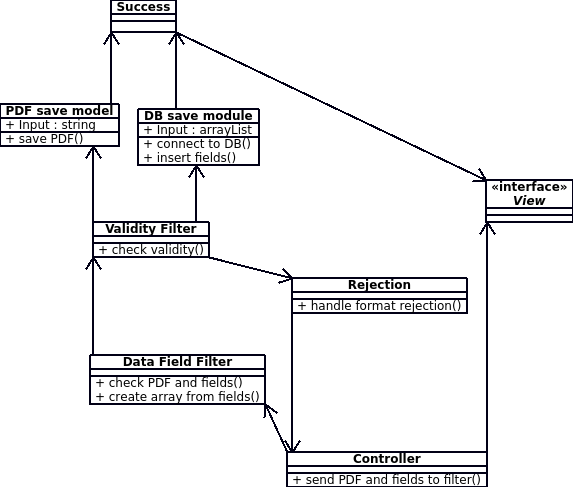
\includegraphics[width=0.8\textwidth]{diagrams/class_diagram.png}
\caption{Digital class diagram}
\label{fig:class_diagram}
\end{figure}
\subsection{Patterns}
MVC due to the technology and pipe \&  filter to filter the data and due to the modifiability requirement.
\subsection{Tactics}
\subsubsection{Modifiability}
\begin{itemize}
\item Increase semantic cohesion
\item Decrease coupling
\item Split modules
\end{itemize}

\subsubsection{Performance}
\begin{itemize}
\item Write optimal code
\end{itemize}

\subsubsection{Availability}
\begin{itemize}
\item Our code should not crash the customer's system, but it's their responsibility that the system is available.
\end{itemize}

\subsubsection{Interoperability}
\begin{itemize}
\item The technology and tools we're using should be sufficient to ensure interoperability.
\end{itemize}

\subsubsection{Readability}
\begin{itemize}
\item We will follow the clean coding principle and use camelCase coding. Refer to \ref{Templates and Standards section} Templates and Standards section on page \pageref{Templates and Standards section}
\end{itemize}

\subsection{Changes to the architecture}
When we started to implement the system we quickly found out that the we had architectural drift because the architecture we designed in the start didn't fit well into the web api framework. After we got an overview of the system we had change the architecture to a MVC pattern. 
\begin{figure}[H]
\centering
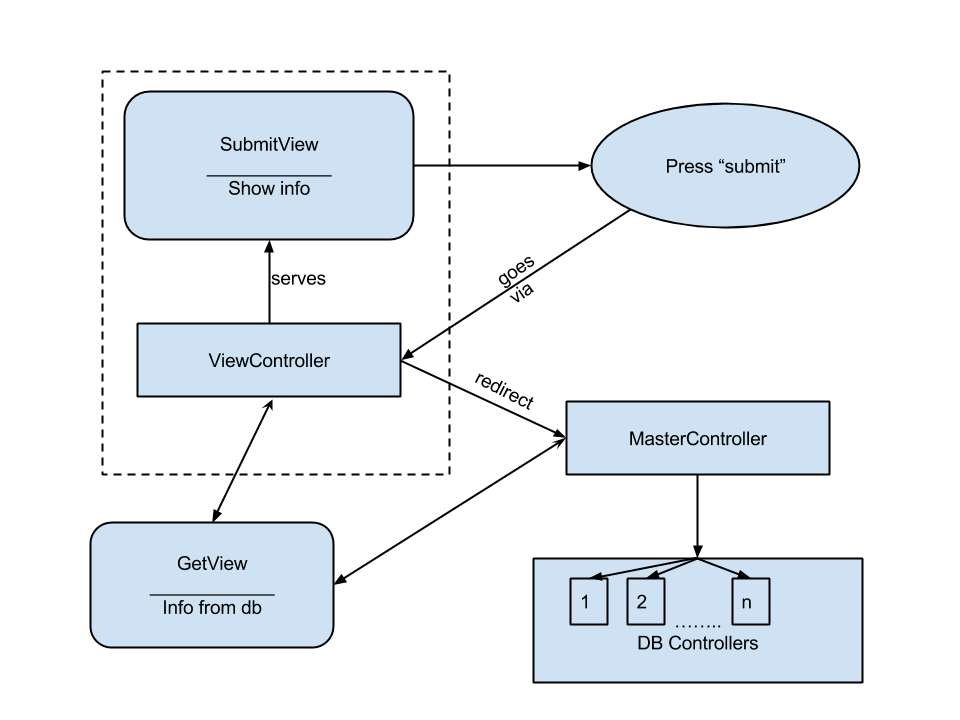
\includegraphics[width=0.8\textwidth]{images/architecture03_revised1.png}
\caption{New diagram showing the information flow}
\label{fig:info_flow}
\end{figure}
We tried to follow this MVC pattern when we implemented the system, however we quickly found out that the getView-Controller was not necessary.
\begin{center}
\begin{figure}[H]
\centering
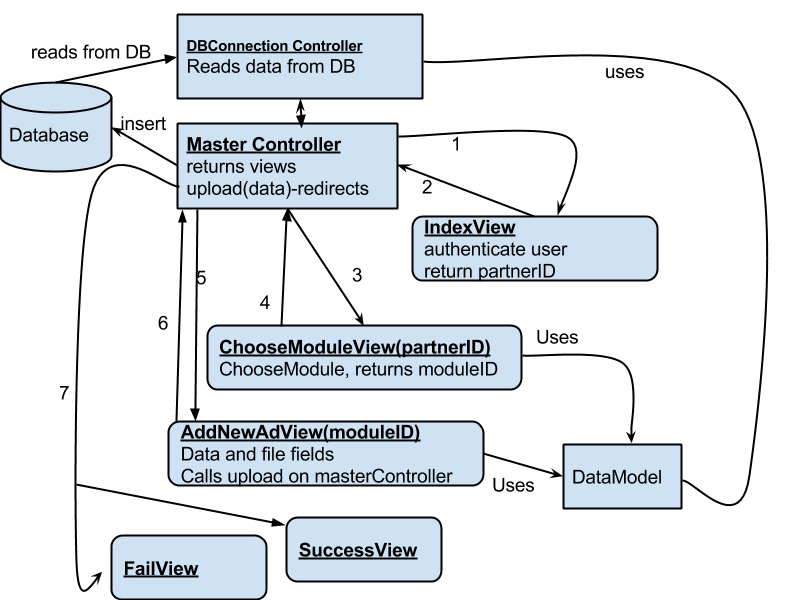
\includegraphics[width=0.8\textwidth]{images/architecture_final01.png}
\caption{The final architecture}
\caption*{6 calls the upload method with files and data\\
7 is the upload method redirecting either to a FailView or a SuccessView}
\label{fig:architecture}
\end{figure}
\end{center}


%Sprints 1-3
\section{Sprint 1}

\subsection{Time Frame}
The time frame for Sprint 1 was week 38 and 39. We started the sprint on September 16th with a weekly supervisor meeting, followed by a sprint plan meeting. We finished the sprint on September 27th with a sprint review meeting.

\subsection{Original Plan}
From our Work Breakdown Structure:
\begin{itemize}
	\item Enable display of available products (no GUI is to be implemented)
	\item Listing the next 5 available booking dates for a selected product
	\item Listing modules available for a selected product
\end{itemize}

\subsection{Revised Plan}
At the sprint plan meeting, we planned the following for this sprint:
\begin{itemize}
	\item Stuff
\end{itemize}

\subsection{Development}
The development started off with the creation of an ASP.NET MVC project. In this project we created data objects for the 

\subsection{Other Work}
In addition to the development, we also completed a draft of the outline for this report and improved on our architectural documentation.

\subsection{Backlog}
What we planned for the sprint that we either did not complete, get time to start, or that was simply pushed back

\subsection{Retrospective}
How we feel about the sprint.
\section{Sprint 2}

\subsection{Time Frame}
The time frame for Sprint 2 was week 40 and 41. We started the sprint on September 30th with a weekly supervisor meeting, followed by a sprint plan meeting. We finished the sprint on October 11th with a sprint review meeting.

\subsection{Original Plan}
From our Work Breakdown Structure, we had the following tasks planned for this sprint:
\begin{itemize}
	\item Receiving pdf-file and save in correct folder
	\item Putting accompanying data in Webassistenten database (table “prospekt”)
	\item Checking accompanying data for required fields
	\item Placing an order in the internal order system
\end{itemize}

Additionally, the following tasks were carried from the previous sprint:
\begin{itemize}
	\item Database connection interface
	\item Database submission logic
\end{itemize}

\subsection{Revised Plan}
At the sprint plan meeting, we planned the following for this sprint:
\begin{itemize}
	\item Set up Entity Framework
	\item Modify start page
	\item Implement saving of pdf-files
	\item Prepare report for midterm delivery
\end{itemize}

\subsection{Development}
At the end of the first sprint, we received a database dump from the customer. The majority of sprint 2 development was centered around setting up a connection to this database through Entity Framework.

Near the end of sprint 2, we realized that we had created the wrong type of project. We had missed the fact that the solution was supposed to use Web API, and had created an MVC project. Some time was therefore spent creating a new Web API project, and porting the code from the previous project into the new one.

\subsection{Other Work}
The deadline for the mid term delivery of the report was originally October 14th, but was at one point in time moved to October 8th. This date coincided with the middle of sprint 2, so a relatively big part of the sprint was spent preparing the report for this delivery. When the deadline was moved back to its original date, more time was spent on improving the report.

\subsection{Backlog}
What we planned for the sprint that we either did not complete, get time to start, or that was simply pushed back.

\subsection{Customer Meeting}
<Add important notes from the customer meeting here, as well as new conclusions made>

\subsection{Retrospective}
<How we feel about the sprint. What we learned, what we are satisfied with, and what we are dissatisfied with.>
\chapter{Sprint 3}

\section{Time Frame}
The time frame for Sprint 3 was week 42 and 43. We started the sprint on October 14th with a weekly supervisor meeting, followed by a sprint plan meeting. We finished the sprint on October 25th with a sprint review meeting.

\section{Original Plan}
From our Work Breakdown Structure:
\begin{itemize}
	\item Database communication interface
	\item Version control system
	\item Bugfixing
	\item Testing
\end{itemize}

\section{Revised Plan}
At the sprint plan meeting, we planned the following for this sprint:
\begin{itemize}
	\item None
\end{itemize}
We had originally planned to be fixing and polishing the finished product, but due to the issues we encountered many of the original planned tasks were pushed to Sprint 3. Sprint 3 thus became a "finish everything that needs to be finished"-Sprint.

\section{Development}
We created the master controller which communicated with the database through the entity framework, it also took care of passing models to the view(s) and handle user request. This master controller was a MVC-type controller which is mostly used as a prototype and for us to test that the data we submit actually reached the system.

\section{Other Work}
After creating and finishing the master controller, the final architecture was made to reflect the implementation of the system. We had architectural erosion due to the framework working differently from what we expected.

The first Friday of this sprint we attended a technical writing course organized by the course staff, where we received pointers on writing our report. These included both general tips as well as concrete improvements for our report specifically.

We started to create the documentation for the customer in Doxygen by XML commenting our code (this was done by adding three slashes "///" in front of all the methods). Doxygen read the implemented code and created the documentation document in HTML. 

\section{Backlog}
Originally we planned to finish the product in Sprint 3, however the we had a lot of issues/problems in both Sprint 1 and 2 so we couldn't start implementing code before Sprint 3. However when the problems were sorted out we actually got down to implementing and communicate with the database. We created a MVC controller of the assignment so we were able to test database connection - insert/select and various other SQL commands via the EF. This MVC controller let us check how the implementation works and gave us a better overview of the framework we were using. However the assignment was to create a Web API controller, so we had to convert it.


\section{Customer Meeting}
We decided to not have a customer meeting for sprint 3 due to our customer Asle not being physically available. Asle was on a 3 weeks vacation in Spain for this period, and we didn't feel the necessity to go to the trouble of setting up a video conference.
However we felt that we had control of the implementation or knew how to fix the issues we stumbled upon. We didn't have much to show either, because we were in the middle of implementing the MVC controller.

\section{Retrospective}
Sprint 3 was a good Sprint for us, we felt that we actually was able to understand the framework and that we actually progressed forward. We was able to communicate with the database, modify rows inside tables, insert data into tables etc.
We also figured out how to serve view (.cshtml) files as webpages through the IIS express by launching the project via VS, and how these views were connected to the controllers. This was enough for us to be able to invoke methods in our controllers, which was heavily used for testing that our written code worked as expected.



\subsection{Tests}

\section{Evaluation}


\section{Conclusion and future work}

\begin{center}
  \begin{tabular}{| l  c  b{5cm}|}
    \hline
    Role & Name & Responsibility \\ \hline 
    Scrum Master & Truls Hamborg &  Scrum master/process manager leads the stand-up meeting. Makes sure the team follows the agreed-upon process. \\ \hline
    Documentation Manager & Truls Hamborg &  Ensures documentation coherency. \\ \hline
    Product Owner (scrum role) & Adressa & The customer, owns the product\\ \hline
    Lead coder & Erlend Sigholt & Oversees coding conventions and makes sure we follow the "clean coding" principles. \\ \hline
    Secretary & Erlend Sigholt & Takes notes during meeting(s) \\ \hline
    Implementation manager & Audun Skjervold & Takes care of learning the framework and implementation of the code.\\ \hline
    Customer and supervisor contact & Hong-Dang Lam & Contact-person for customer and supervisor \\ \hline
    System Architect & Hong-Dang Lam & Create and maintain the architecture of the system \\
    \hline
  \end{tabular}
\end{center}


 
 
%%%Technology
%%%\documentclass[12pt, a4paper]{article} 
 
\usepackage[utf8]{inputenc}
 
 
\usepackage{geometry} % to change the page dimensions
\geometry{a4paper} % or letterpaper (US) or a5paper or....
 
\usepackage{graphicx} % support the \includegraphics command and options
 
\usepackage{booktabs} % for much better looking tables
\usepackage{array} % for better arrays (eg matrices) in maths
\usepackage{paralist} % very flexible & customisable lists (eg. enumerate/itemize, etc.)
\usepackage{verbatim} % adds environment for commenting out blocks of text & for better verbatim
\usepackage{subfig} % make it possible to include more than one captioned figure/table in a single float
% These packages are all incorporated in the memoir class to one degree or another...
 
 
 
\usepackage{amsmath, amssymb}% for mathematical symbols
\usepackage[colorlinks=true,linkcolor=black, urlcolor=blue]{hyperref} % for hyperreferences with black color
%\usepackage[T1]{fontenc} % Uncomment for norwegian document
%\usepackage[norsk]{babel} %
 
%%% HEADERS & FOOTERS
\usepackage{fancyhdr} % This should be set AFTER setting up the page geometry
\pagestyle{fancy} % options: empty , plain , fancy
\renewcommand{\headrulewidth}{0pt} % customise the layout...
\lhead{}\chead{}\rhead{}
\lfoot{}\cfoot{\thepage}\rfoot{}
 
%%% SECTION TITLE APPEARANCE
\usepackage{sectsty}
\allsectionsfont{\sffamily\mdseries\upshape} % (See the fntguide.pdf for font help)
% (This matches ConTeXt defaults)
 
%%% ToC (table of contents) APPEARANCE
\usepackage[nottoc,notlof,notlot]{tocbibind} % Put the bibliography in the ToC
\usepackage[titles,subfigure]{tocloft} % Alter the style of the Table of Contents
\renewcommand{\cftsecfont}{\rmfamily\mdseries\upshape}
\renewcommand{\cftsecpagefont}{\rmfamily\mdseries\upshape} % No bold!

\begin{document}

\section{Technology}

\subsection{Windows 7, 8}
Microsoft Windows 7 and - 8 are operating systems by the Microsoft Corporation. They logically provide good support for .NET developments, seeing as .NET targets the Windows platform and is made by Microsoft. Visual Studio is made for Windows, and was our main IDE, so all team members had access to PCs with Windows installed.

\subsection{Ubuntu Linux}
This OS is perhaps the most widely used distribution of Linux, developed by Canonical Ltd. It provides good support for many development tools, except of course Windows development. However we did find support for using it for some Windows development.
This operating system was used by one team-member on a laptop, when working on-site at NTNU. For coding, Mono with MonoDevelop was used, while other tasks were mostly unaffected. The operating system provides good support for other parts of the process, such as Git and \LaTeX.

\subsection{Mac OSX}
%TODO

\subsection{Visual Studio 2012}
Visual Studio is Microsofts IDE for development for their platforms. This is the main IDE we developed the framework on, seeing as it has very good integration with C\# and .NET platforms, which we were required to use.

\subsection{.NET and Mono}
We were required to use ASP .NET MVC for our framework. ASP .NET MVC is a framework for web applications which enables the use of the Model View Controller (MVC) pattern. It is part of Microsofts .NET Framework suite, which is the preferred way of interactiong with Windows systems and OSes.

Mono is the open source-, cross-platform version of the .NET suite, which we used when not developing on Windows machines. It is available both for Windows, OS X, most Linux Distributions, Android, and various other operating systems.

\subsection{MonoDevelop}
This is an open source IDE for development with Mono, available for OS X and most Linux distributions. This was the IDE used when not developing on Windows machines.

\subsection{LaTeX}
We quickly chose \LaTeX \ for our typesetting. It being the de-facto standard for academic typesetting, with good support for both code snippets, tables, references and bibliography.

Most of our group also had at least some experience using it, and some were quite experienced, which made the choice easier.

\subsection{Git}
For our version control and source repository, we chose Git. This because we had most experience with it, and found it easy to set up via GitHub (where we all had accounts already). It also has the advantage of being distributed, so we could avoid a single point of failure, and having a staging area where one can selectively commit files according to whether they're ready or not, instead of risking accidental changes which might break something.

Both the source code and the entirety of the report source files were stored on GitHub, since both would be catastrophical to lose, and were quite important to have under version control in case we needed to track problematic changes.

\subsection{Trello}
To support our agile process and sprints, we used Trello for planning and control of workflow. It is an online Kanban Board tool, where we can create work packages and issues, while tracking who does what, and tracking backlog, finished modules, and work in progress.

\subsection{Web API}
%TODO

\subsection{Dropbox}
\href{http://www.dropbox.com}{Dropbox} is a syncing service that let you choose a local folder on your machine that will be synced to the cloud. Dropbox lets you share folders and files inside a shared Dropbox folder.

We used Dropbox for sharing and synchronizing internal documents that usually were only useful for a limited time, but might be referenced later.

\subsection{Google Drive}
\href{https://drive.google.com/}{Google Drive} is Google's office pack. The difference between Drive and other office solutions (like Microsoft Office , OpenOffice/LibreOffice) is that Drive exist in the cloud and lets the user simultaneously work on a document.

Google Drive was used for simultaneous collaboration on documents, where the content was up for discussion, or it was advantageous to see what the others where writing.

\end{document}	%%%TODO: Comment in this when technology file is complete, and begindocument is removed

\end{document}